\documentclass[11pt]{article}

\usepackage{latexsym}
\usepackage{amssymb}
\usepackage{amsthm}
\usepackage{enumerate}
\usepackage{amsmath}
\usepackage{cancel}
\usepackage{graphicx}
\numberwithin{equation}{section}

\setlength{\evensidemargin}{.25in}
\setlength{\oddsidemargin}{-.25in}
\setlength{\topmargin}{-.75in}
\setlength{\textwidth}{6.5in}
\setlength{\textheight}{9.5in}
\newcommand{\due}{November 28th, 2016}
\newcommand{\HWnum}{1}
\newcommand{\grad}{\bold\nabla}
\newcommand{\vecE}{\vec{E}}
\newcommand{\scrptR}{\vec{\mathfrak{R}}}
\newcommand{\kapa}{\frac{1}{4\pi\epsilon_0}}
\newcommand{\emf}{\mathcal{E}}
\newcommand{\unit}[1]{\ensuremath{\, \mathrm{#1}}}
\newcommand{\real}{\textnormal{Re}}
\newcommand{\Erf}{\textnormal{Erf}}
\newcommand{\sech}{\textnormal{sech}}
\newcommand{\scrO}{\mathcal{O}}
\newcommand{\levi}{\widetilde{\epsilon}}
\newcommand{\partiald}[2]{\ensuremath{\frac{\partial{#1}}{\partial{#2}}}}
\newcommand{\norm}[2]{\langle{#1}|{#2}\rangle}
\newcommand{\inprod}[2]{\langle{#1}|{#2}\rangle}
\newcommand{\ket}[1]{|{#1}\rangle}
\newcommand{\bra}[1]{\langle{#1}|}





\begin{document}
\begin{titlepage}
\setlength{\topmargin}{1.5in}
\begin{center}
\Huge{Physics 3320} \\
\LARGE{Principles of Electricity and Magnetism II} \\
\Large{Professor Ana Maria Rey} \\[1cm]

\huge{Homework \#\HWnum}\\[0.5cm]

\large{Joe Becker} \\
\large{SID: 810-07-1484} \\
\large{\due} 

\end{center}

\end{titlepage}



\section{Problem \#1}
\begin{enumerate}[(a)]
    \item
    For a waveguide whose cross-section is an equilateral triangle whose vertices are at
    $$(x,y) = \left\{(0,0),(a,a/\sqrt{3}),(a,-a/\sqrt{3})\right\}$$
    we can verify that the function
    $$\psi_{mn} = \sin\frac{l\pi{x}}{a}\sin\frac{(m-n)\pi{y}}{a\sqrt{3}} + \sin\frac{m\pi{x}}{a}\sin\frac{(n-l)\pi{y}}{a\sqrt{3}} + \sin\frac{n\pi{x}}{a}\sin\frac{(l-m)\pi{y}}{a\sqrt{3}}$$
    where $l\equiv-m-n$ satisfy the TM boundary conditions as shown in figure \ref{Triangle}
    \begin{figure}
        \centering
        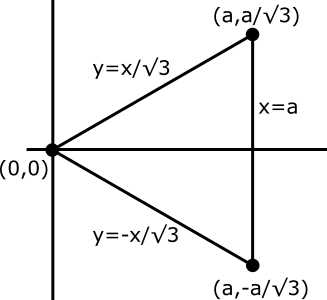
\includegraphics[width=0.5\textwidth]{Triangle.png}
        \caption{Equilateral triangle waveguide geometry.}
        \label{Triangle}
    \end{figure}
    If we recall the result from homework 7 we see that 
    $$\psi_{nm}(a,y) = \cancelto{0}{\sin{l\pi}}\sin\frac{(m-n)\pi{y}}{a\sqrt{3}}
        + \cancelto{0}{\sin{m\pi}}\sin\frac{(n-l)\pi{y}}{a\sqrt{3}}
        + \cancelto{0}{\sin{n\pi}}\sin\frac{(l-m)\pi{y}}{a\sqrt{3}} = 0$$
     and
    \begin{align*}
        \psi_{nm}(x,x/\sqrt{3}) &= \sin\frac{l\pi{x}}{a}\sin\frac{(m-n)\pi{x}}{3a}
            + \sin\frac{m\pi{x}}{a}\sin\frac{(n-l)\pi{x}}{3a}
            + \sin\frac{n\pi{x}}{a}\sin\frac{(l-m)\pi{x}}{3a}\\
        &= \frac{1}{2}\left[\cos\left(\frac{\pi{x}}{3a}(4m+2n)\right) - \cos\left(\frac{\pi{x}}{3a}(4m+2n)\right)\right.\\
        &\qquad+\cos\left(\frac{\pi{x}}{3a}(2m-2n)\right) - \cos\left(\frac{\pi{x}}{3a}(2m-2n)\right)\\
        &\qquad+\left.\cos\left(\frac{\pi{x}}{3a}(4n+2m)\right) - \cos\left(\frac{\pi{x}}{3a}(4n+2m)\right)\right]= 0
    \end{align*}
    Note that for the final boundary condition we can use the result from above and the fact
    that sine is a odd function to see
    \begin{align*}
        \psi_{nm}(x,-x/\sqrt{3}) &= \sin\frac{l\pi{x}}{a}\sin\frac{-(m-n)\pi{x}}{3a}
            + \sin\frac{m\pi{x}}{a}\sin\frac{-(n-l)\pi{x}}{3a}
            + \sin\frac{n\pi{x}}{a}\sin\frac{-(l-m)\pi{x}}{3a}\\
        &= -\left(\sin\frac{l\pi{x}}{a}\sin\frac{(m-n)\pi{x}}{3a}
            + \sin\frac{m\pi{x}}{a}\sin\frac{(n-l)\pi{x}}{3a}
            + \sin\frac{n\pi{x}}{a}\sin\frac{(l-m)\pi{x}}{3a}\right)\\
        &= -\psi_{nm}(x,x/\sqrt{3}) = 0
    \end{align*}
    So we see that all TM boundary conditions are met.

\item
    There exists a further set of TM modes, but not the modes described by the bisected 
    equilateral triangular waveguide described in part (a). Note that we already have met the
    boundary condition for the full equilateral triangle with an additional boundary 
    condition that $\psi_{mn}(0,y) = 0$.

   

\item
\end{enumerate}

\pagebreak

\section{Problem \#2}
\begin{enumerate}[(a)]
\item
\item
\end{enumerate}

\end{document}

